\documentclass[conference]{IEEEtran}
\IEEEoverridecommandlockouts
% The preceding line is only needed to identify funding in the first footnote. If that is unneeded, please comment it out.
\usepackage{cite}
\usepackage{amsmath,amssymb,amsfonts}
\usepackage{algorithmic}
\usepackage{graphicx}
\usepackage{textcomp}
\usepackage{url}
\usepackage{multicol}

\begin{document}

\title{Defining C-ITS Reference Architecture* \\
  {\footnotesize \textsuperscript{*}Industrial Experience Report}
  \thanks{Funded by European Union Commission , 723311.}
}

\author{
  \IEEEauthorblockN{Priyanka Karkhanis,
    Mark van den Brand, Saurab Rajkarnikar}
  \IEEEauthorblockA{Eindhoven University of Technology\\
    Eindhoven, The Netherlands\\
    Email: p.d.karkhanis@tue.nl,
    M.G.J.v.d.Brand@tue.nl,
    s.rajkarnikar@tue.nl}
}

\maketitle


\begin{abstract}
C-ITS (Cooperative Intelligent Transport Systems) is an initiative to facilitate cooperative, connected and automated mobility.
It is based on the concept of System of Systems and promotes a new way of thinking for solving grand challenges where the interactions of technology, policy and economics are the primary drivers.

The C-ITS domain comprises widely spread systems like traffic management systems, traffic light controllers, or vehicle on-board units.
Such complex and heterogeneous systems have independent uses but demand a strategy to facilitate their convergence.

The main objective of C-ITS is to define an integrated architecture based on a number of existing C-ITS projects.
The architecture provides a way to standardize and a unifying modeling approach by means of a common language that can be reused by other organizations to guide their internal development processes.
The architecture and its concepts are based on the conceptual model of the ISO/IEC/IEEE 42010 \cite{iso42010} international standard for architecture descriptions of systems, System of Systems and software.
It defines architecture viewpoints for C-ITS systems and uses the concept of architecture perspective for shaping these architecture viewpoints.
In this paper we present the methodology used for defining the C-MobILE reference architecture.
We demonstrate this by means of the C-MoBILE reference architecture, which allows large scale demonstrations of integrations of C-ITS systems across Europe.
\end{abstract}

\begin{IEEEkeywords}
C-ITS, ITS, architecture framework, transportation
\end{IEEEkeywords}


\section{Introduction}

The European Parliament in it's directive 2010/40/EU \cite{ec} defines Intelligent Transport System(ITS) as "systems in which information and communication technologies are pplied in the field of road transport, including infrastructure, vehicles and users, and in traffic management and mobility management, as well as for interfaces with other modes of transport.
"It can be further stated as systems which aims in making transportation safe and economoical by combining data from the vehicles and other sensors on the roadway together with weather information.
Cooperative-Intelligent Transport System(C-ITS) \cite{c-its} adds upon ITS by providing ways for connected vehicles to interact with other connecte vehicles or any infrastructure such as a Road Side Unit.
This interaction is where the term cooperatives comes from.
In this scenario the vehicles can act as sensors as well.

The C-MobILE (Accelerating C-ITS Mobility Innovation and deployment in Europe) project is a European Union (EU) project that spans across eight C-ITS equipped deployment sites and regions with more than 37 participating institutes and companies.
The C-ITS domain covers not only software/system engineering field, but also traffic engineering, civil engineering, information technology etc., which require a unified definition of architecture for the C-ITS domain.
It aims to make road transport safe and efficient while decreasing casualties and serious injuries on European roads.
The eight C-ITS equipped deployment sites already have some C-ITS services through various projects that took place in the past.
However, many of these are not interoperable.
Thus, C-MobILE plans to become a common approach that ensures interoperability with seamless service and become a basis for large scale deployment in Europe.
It is working with various public and private stakeholders while carrying out and developing cost effective business models particularly from the end user’s perspective.
To help reach the project goals, a good architecture, capable of being deployed to whole Europe is needed.
The architecture definition process in C-MobILE has been defined to support the following sub-goals:

\begin{itemize}
  \item To analyse existing C-ITS architectures to provide common concepts and vocabulary.
  \item To identify a set of patterns that have been detected (or applied implicitly) during the analysis of existing C-ITS architectures and their implementations.
  \item To create a C-ITS reference architecture that enables pan-European interoperability of C-ITS (concrete/implementation) architectures based on the generalization of existing C-ITS architectures.
  \item To define an implementation architecture specifying components and their relationships (interfaces) guided and constrained by the C-ITS reference architecture.
  \item To identify service-relevant parts of the architecture and define services based on the business analysis.
\end{itemize}

C-ITS projects that are/were deployed and are considered for C-MobILE project are: The Dutch C-ITS Reference Architecture \cite{ditcm}, Spookfiles A58\footnote{Shockwave traffic jams a58. \url{http://www.spookfiles.nl/shockwave-traffic-jams-a58}.}, Praktijkproef Amsterdam\footnote{Praktijkproef amsterdam. \url{https://www.rijkswaterstaat.nl/zakelijk/innovatie-en-duurzame-leefomgeving/innovatie/wegeninnovaties/praktijkproef-amsterdam.aspx}.}, C-ITS Corridor\footnote{Cooperative its corridor.\url{https://itscorridor.mett.nl/default.aspx}}, MOBiNET\footnote{MOBiNET. \url{http://www.mobinet.eu/}.}, VRUITS\footnote{Improving the safety and mobility of vulnerable road users through its applications. \url{https://cordis.europa.eu/project/rcn/186986_en.html}.}, CONVERGE\footnote{Converge. \url{https://converge-online.de/}}, COMPASS4D\footnote{Compass4d. \url{http://ertico.com/projects/compass4d/}.}, NordicWay\footnote{Nordicway. \url{http://vejdirektoratet.dk/EN/roadsector/Nordicway/Pages/Default.aspx}.} and ARC-IT\footnote{Arc-it version 8.1. \url{https://local.iteris.com/arc-it/}.}.


\section{Problem Statement}

C-MobILE architecture aims for large scale demonstration project across various pilot sites.
These various deployment sites either have their own defined ITS architecture.
These various pilot sites have their own multidisciplinary approach towards their specific deployed strategy.
These architectures comprise of different design patterns in the form of informal notations.
There is no standard notation to help in merging these architectures into a silo-based architecture.
An architecture that should not change the existing technology but to harmonize with other existing architectures.
Without the common C-ITS architecture framework, different categorizations and ad-hoc notations have been used in the existing C-ITS architectures.
Hence, this demands a standardized approach to consolidate and integrate existing architectures ensuring the concerns such as interoperability, security, availability, and maintainability shall also be addressed.

\begin{figure*}[!t]
  \centering
  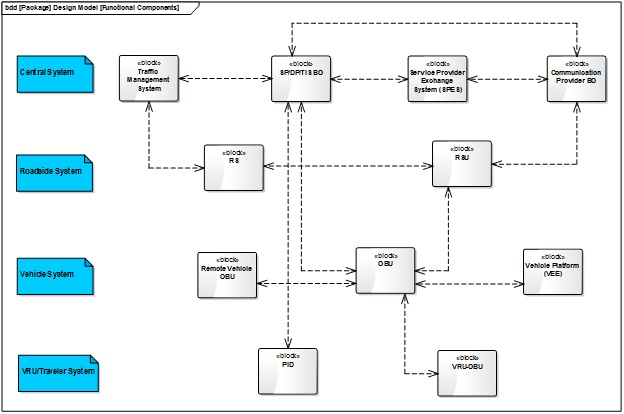
\includegraphics[width=0.8\textwidth]{functional_vp}
  \caption{Functional model capturing functional viewpoint of the C-ITS systems for C-MobILE.}
  \label{functional}
  \centering

\end{figure*}


\section{Methodology}

We considered various C-ITS projects as mentioned in introduction section.
Apart from these C-ITS architectures, we considered current ongoing ITS implementation for the deployed sites involved in C-MobILE.
We applied reverse architect approach by extracting the systems, protocols, networks, technology details etc.
from all of these architectures manually.
A repository has been constructed consolidating all the necessary and required information from existing architectures.
A thorough analysis was done to extract the commonalities, but not leaving behind their specific implementation details.
As a well-defined architecture framework is considered to be an important part of any architecture description \cite{archframework}, we defined an architecture framework for the C-ITS domain \cite{ITSCongress}.
The architecture frameworks facilitate communication and cooperation between different stakeholders during architecting and building complex systems such as C-ITS.
Many different stakeholders with their interweaving concerns require a systematic approach for addressing complexity and full lifecycle of the system.
To put architecture framework and architecture description concepts in context, we extend the conceptual model of the ISO/IEC/IEEE 42010\cite{iso42010} architecture framework.
The C-ITS architecture framework specifies stakeholders, their concerns, viewpoints, model kinds, and correspondence rules.
C-ITS architects can use an architecture framework to represent the C-ITS reference architecture, concrete, implementation and deployed site architectures.

To design C-MobILE architecture framework strategy, the architecture process has been split into three parts: In the first design phase, the reference architecture has been created by analysing existing architectures, described in section IV.
In parallel, use-cases, business-cases, and requirements to the C-MobILE system have been collected.
During the second design phase, the reference architecture will be used to create the medium-level architecture.
Furthermore, services, interfaces, and concepts will be described to provide a guideline for the final stage.
In the third design phase, interfaces and concepts will be described in detail to create a low-level implementation architecture.
We propose to use Systems Modelling Language (SysML) diagram types for architectural notations of the C-ITS architectures.
The SysML is a general purpose modelling language for engineering systems and consists of structure diagram, requirement diagram, and behavior diagram.
The architecture framework and the same modelling approach can enable common language and will be reused for the next deployment projects.
Furthermore, organizations can use the architecture to guide their internal development process as it reflects a common understanding of how the (future) ITS landscape will evolve.


\section{C-MobILE Reference Architecture}

C-MobILE Reference Architecture focuses more on an abstract level and use “black box” approach wherever possible.
It describes various systems at a high level in the form of models using SysML.
The SysML Block Definition Diagram and Internal Block Diagram are used to represent the models for the reference architecture at an abstract level providing base level information to architects.
However, due to the heterogeneous nature of such interfaces this will not be possible for all interfaces of the architecture.
For example, there exists several competing standards for roadside infrastructure to communicate with traffic management centers.
C-MobILE reference architecture does neither have the resource nor the intention to change/redefine all those standards.
Instead, at high level we highlight the common systems, their interfaces and protocols by considering various existing projects to ensure interoperability.

As a result of the architecture analysis and reverse architecting process, we have extracted the reference architecture from various existing reference architectures, which was consistent with the DITCM reference architecture.
The structure of a system is captured in functional structure models using SysML BDD by categorizing into systems and decomposing a system into subsystems.
A system defines the functionality and functional data flow interfaces between systems that are required to support a particular ITS application.
Functional model digram is illustrated in figure \ref{functional} for capturing functional viewpoint.



Functional viewpoint describes the system’s runtime functional elements, their responsibilities, interfaces, and primary interactions.
The functional view conforms to the functional viewpoint, helps the system’s stakeholders understand the system structures, and has an impact on the system’s quality properties.
The system structure is captured in functional models using SysML block definition diagram (BDD) and by categorizing into systems and decomposing a system into subsystems.
A system defines the functionality and functional data flow interfaces between systems that are required to support a particular ITS application.
Information flows depict the exchange of information between subsystems.


\section{Conclusions and Further Work}

In this paper, we have presented the methodology used for defining the C-MobILE reference architecture.
We have analysed existing C-ITS architectures, especially CONVERGE, MOBiNET, and Dutch C-ITS Reference Architecture, to define common concepts and vocabulary for the C-MobILE reference, concrete, and implementation architectures The different architectures from the pilot sites are used as an input for defining a single homogeneous reference architecture in line with current standards which will be further refined.
We adapted reverse architect approach manually for extracting the components, systems, technological details etc.
The next step is to automate this approach as well intended to provide benefit for system architects and stakeholders.


\section*{Acknowledgment}

The C-MobILE project has received funding from the European Union’s Horizon 2020 research and innovation programme under grant agreement No 723311.


\begin{thebibliography}{00}

    \bibitem{ec} European Commission. Directive 2010/40/eu of the european parliament and of the council.
    \bibitem{ecits} European Commission. Intelligent transport systems. \url{https://ec.europa.eu/transport/themes/its/c-its_en}.
    \bibitem{ditcm} Marcel van Sambeek, Frank Ophelders, Tjerk Bijlsmaand Borgert van der Kluit, Oktay Turetken, Rik Eshuis, Kostas Traganos, and Paul Grefen. Towards an architecture for cooperative-intelligent transport system (c-its) applications in the netherlands. Available at \url{ https://www.researchgate.net/publication/313580768_Towards_an_Architecture_for_Cooperative-Intelligent_Transport_System_C-ITS_Applications_in_the_Netherlands}.

    \bibitem{iso42010} ISO/IEC/IEEE Systems and software engineering -- Architecture description," in ISO/IEC/IEEE 42010:2011(E) (Revision of ISO/IEC 42010:2007 and IEEE Std 1471-2000) , vol., no., pp.1-46, Dec. 1 2011 doi: 10.1109/IEEESTD.2011.6129467
    \bibitem{archframework}Emery, D., and Rich H. Every architecture description needs a framework: Expressing architecture frameworks using ISO/IEC 42010. Software Architecture, 2009 \& European Conference on Software Architecture. WICSA/ECSA 2009. Joint Working IEEE/IFIP Conference on. IEEE, 2009.
    \bibitem{ITSCongress}Raul Ferrandez, Yanja Dajsuren, Priyanka Karkhanis, Manuel Fünfrocken, Marcos Pillado. C-MobILE C-ITS Reference Architecture. ITS World Congress 2018 (unpublished).
    \bibitem{c-its}A. Festag, "Cooperative intelligent transport systems standards in europe," in IEEE Communications Magazine, vol. 52, no. 12, pp. 166-172, December 2014.  doi: 10.1109/MCOM.2014.6979970

\end{thebibliography}


\end{document}
